\newsection{Modello di Sviluppo}
Come \gl{modello di ciclo di vita} da applicare abbiamo scelto il \gl{modello incrementale}. La scelta di un modello di sviluppo specifico è indispensabile per organizzare e controllare lo svolgimento delle attività necessarie per la realizzazione del prodotto richiesto. Il totale abbiamo determinato che effettueremo 16 incrementi. Nella sezione specifica di ogni periodo è indicato quanti incrementi verranno effettuati.

\subsection{Modello incrementale}
Il modello di sviluppo incrementale prevede rilasci in sequenza, ognuno con nuove caratteristiche rispetto al precedente. Si comincia dalle funzionalità corrispondenti ai requisiti fondamentali per poi passare ai requisiti opzionali. I requisiti vengono quindi suddivisi nei vari incrementi in base alla loro priorità, rendendo quindi anche la consegna del prodotto incrementale.
Suddividere le attività in questi incrementi porta ad una gestione semplificata e maggiormente controllabile delle risorse e dei tempi.\\
Durante ogni \gl{incremento} non è possibile modificare i requisiti decisi, tuttavia è possibile aggiungere requisiti da sviluppare nei successivi incrementi.
I vantaggi principali consistono nel poter valutare dopo ogni incremento i miglioramenti fatti e la possibilità di avere anticipatamente una versione incompleta ma funzionante del prodotto. \\
\begin{center}
\begin{figure} [H]
	\centering
	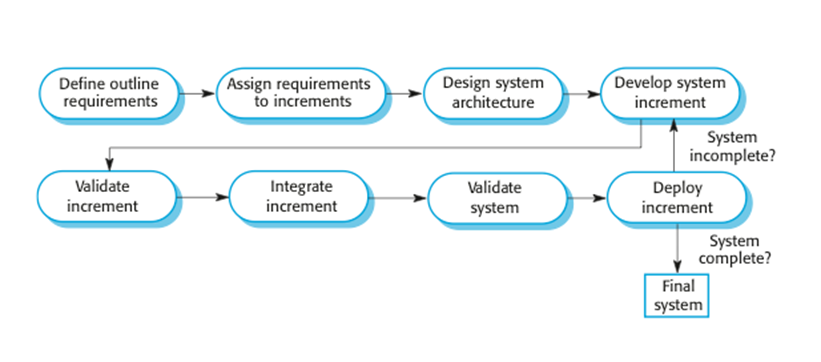
\includegraphics[scale=0.65]{Img/Schema_modello_incrementale}
	\caption{Figura 3.1: Modello incrementale}\label{}
\end{figure}
\end{center}
\subsection{Pianificazione incremento}
Ogni incremento sarà considerato come un \textit{periodo}. Ogni periodo è composto dalle attività specificate nei corrispondenti diagrammi di Gantt e strutturato come segue:
\begin{itemize}
\item \textbf{Riunione iniziale:} all'inizio del periodo si svolgerà una riunione con tutti i membri del gruppo, per decidere le attività da svolgere. Ogni attività verrà quindi assegnata ad uno o più membri del team;
\item \textbf{Svolgimento delle attività:} vengono svolte le attività discusse in precedenza. In caso sorgano dei problemi, se ne discuterà con gli altri membri del team per trovare la soluzione ottimale;
\item \textbf{\gl{Verifica} e revisione:} si verificano le attività completate, per valutare la loro conformità alle aspettative.
\end{itemize}
La durata di ognuno di questi punti potrebbe variare a seconda della difficoltà delle attività da svolgere o a seconda degli impegni dei membri del team.
\newpage
